% Workshop condensation of the full OpenAdapt technical report
% ("Compile Once, Govern Every Repair: Deterministic Replay for Repeated GUI
% Work", paper/main.tex). This ~8-page version is deliberately reframed around
% the single sharpest finding -- that task-success metrics overstate GUI-agent
% reliability because they score the screen, not the business effect -- and
% defers system depth to the full report. It copies paper/references.bib and
% reuses the exact machine-checked benchmark constants (see paper/check_artifacts.py).
% Venue-agnostic single-column article for now; retarget the class to a chosen
% NeurIPS 2026 workshop style when selected.

\documentclass[10pt]{article}

\usepackage[margin=1in]{geometry}
\usepackage[T1]{fontenc}
\usepackage{lmodern}
\usepackage{booktabs}
\usepackage{amssymb}
\usepackage{microtype}
\usepackage{hyperref}
\usepackage{xcolor}
\usepackage{tikz}
\usetikzlibrary{positioning,arrows.meta,shapes.geometric,fit,backgrounds,calc,decorations.pathreplacing}
\usepackage{pgfplots}
\pgfplotsset{compat=1.13}

\definecolor{oaink}{HTML}{1F2933}
\definecolor{oablue}{HTML}{2563EB}
\definecolor{oagreen}{HTML}{15803D}
\definecolor{oared}{HTML}{B91C1C}
\definecolor{oaamber}{HTML}{B45309}
\definecolor{oagray}{HTML}{E5E7EB}

\hypersetup{
  colorlinks=true,
  linkcolor=black,
  citecolor=blue,
  urlcolor=blue,
  pdftitle={A Green Screen Is Not a Saved Record},
  pdfsubject={Workshop condensation of the OpenAdapt technical report}
}
\newcommand{\system}{OpenAdapt}
\newcommand{\fullreport}{\href{https://github.com/OpenAdaptAI/openadapt-flow}{full technical report}}

\title{A Green Screen Is Not a Saved Record:\\
Effect-Level Verification for Repeated GUI Work}
\author{Richard Abrich\\OpenAdapt (MLDSAI Inc.)\\\texttt{richard@openadapt.ai}}
\date{Workshop draft of July 2026}

\begin{document}
\maketitle

\begin{abstract}
Benchmarks for computer-use and GUI agents report \emph{task success}: an
external oracle inspects the final screen and declares the task done. We argue
this metric systematically overstates reliability for consequential work,
because a rendered success is not a persisted effect. The same green ``Saved''
banner can follow a partial write, a duplicate submission, a stale overwrite, or
a silently rejected transaction. We call the resulting error a \emph{silent
incorrect success} and show it is common and measurable. Injecting seven
persistence faults behind a real HTTP boundary and running each ten times,
screen-only verification silently accepted 50 of 90 fault runs; declaring a
typed effect and checking it against the application's own system of record drove
that to 0 of 90. A companion adversarial study shows the dual failure at the
identity layer: where confusable glyphs (O/0, l/1) make look-alike records
observationally identical, the safe response is to refuse, and our identity
ladder recorded zero false accepts across every configuration. The mechanism is a
demonstration compiler that replays a recorded workflow deterministically and
verifies effects rather than pixels; we summarize it briefly and defer depth to
the full report. Our claim for this venue is narrow and, we think, important:
report silent incorrect success and over-halt alongside task success, and verify
effects at the system of record.
\end{abstract}

\section{Task success scores the screen, not the effect}
\label{sec:intro}

A general computer-use agent observes a screen and chooses the next action with a
model; benchmarks such as WebArena, WorkArena, and OSWorld measure how often such
an agent \emph{completes} a task, judged by an oracle that reads the final state
of the interface \cite{webarena,workarena,osworld}. This is the right question
for breadth on previously unseen tasks. It is the wrong question for the failure
that costs money in production.

Consider the last mile of almost any operational workflow: a form is filled and a
``Save'' button is pressed. The agent, or a recorded script, looks for a green
confirmation banner and stops. A banner is a picture of success. It is not a
saved record. Between the click and the durable write sit optimistic rendering,
partial commits, idempotency hazards, and server-side rejection, any of which can
leave the screen green and the database wrong. When an automation reports success
after such an event, we call it a \emph{silent incorrect success}: no crash, no
timeout, no alert, and a downstream owner who inherits a note in the wrong
patient's chart or a payment posted to the wrong account.

Task-success oracles are, by construction, blind to this class. They read the
same screen the automation trusted. Our position is that any reliability claim
for consequential GUI work must additionally report two quantities: the rate of
silent incorrect success against an \emph{independent} oracle, and the rate of
\emph{over-halt} (refusing when the correct action was in fact available), so
that safety is not obtained by refusing everything. This paper substantiates the
position with a controlled fault study and an adversarial identity study, and
sketches a mechanism that acts on it. The full system, additional substrates
(native Windows UI Automation, macOS, and real-network RDP), and a broader
evaluation are in the \fullreport{}; every number below is bound by a
machine-check to a released benchmark artifact.

\section{The screen is a weak oracle}
\label{sec:oracle}

Deciding whether an observed outcome is correct is the \emph{test-oracle problem}
\cite{barr2015oracle}. GUI automation has quietly standardized on the weakest
available oracle: a screenshot. The end-to-end argument in system design tells us
why this is a mistake---a correctness check belongs at the layer that can
establish the intended property, not at an intermediate one
\cite{saltzer1984end}. For a business transaction, that layer is the system of
record, not the rendered page. The faults that slip past the screen---duplicate
submission, double delivery, stale overwrite---are the same exactly-once and
idempotency hazards long studied in transactional systems
\cite{gray1981transaction}.

\system{} therefore separates two oracles (Figure~\ref{fig:oracle}). A screen
\emph{postcondition} (a banner, a URL change, a stable region) is necessary but
not sufficient. A consequential step additionally declares a typed \emph{effect}
and checks it with an independent verifier that snapshots the system of record
before and after the action---over REST, FHIR, or document state---and returns
confirmed, refuted, or indeterminate. A declared effect without a configured
verifier halts rather than proceeding on trust.

\begin{figure}[t]
\centering
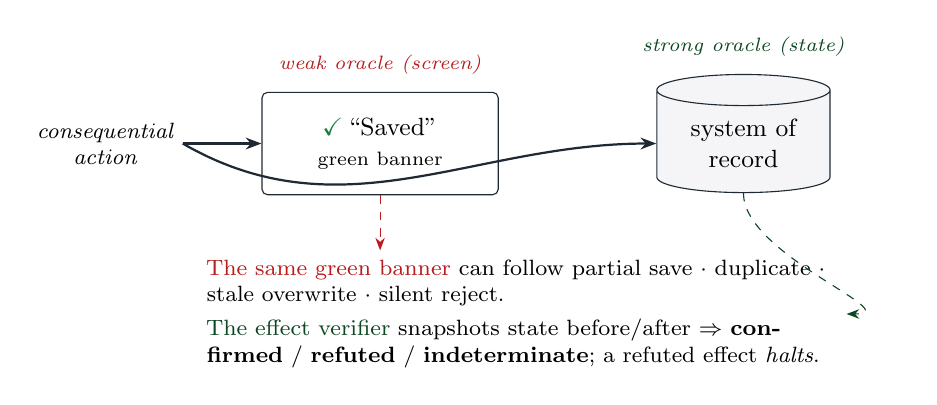
\begin{tikzpicture}[
  font=\small,
  screen/.style={draw=oaink, rounded corners=2pt, minimum width=30mm,
    minimum height=13mm, align=center, fill=white},
  db/.style={draw=oaink, cylinder, shape border rotate=90, aspect=0.28,
    minimum width=22mm, minimum height=15mm, align=center, fill=oagray!40,
    inner sep=1pt},
  ]
  \node[align=center, font=\footnotesize\itshape] (act) {consequential\\action};
  \node[screen, right=10mm of act] (scr)
    {\textcolor{oagreen}{$\checkmark$}\,``Saved''\\\scriptsize green banner};
  \node[db, right=20mm of scr] (db) {system of\\record};
  \draw[-{Stealth[length=2mm]}, thick, oaink] (act) -- (scr);
  \draw[-{Stealth[length=2mm]}, thick, oaink] (act.east) to[out=-30,in=180] (db.west);
  \node[above=1mm of scr, font=\scriptsize\itshape, text=oared] {weak oracle (screen)};
  \node[above=1mm of db, font=\scriptsize\itshape, text=oagreen!55!black] {strong oracle (state)};
  \node[align=left, font=\footnotesize, below=7mm of scr, text width=80mm, xshift=18mm] (gap)
    {\textcolor{oared}{The same green banner} can follow partial save $\cdot$
     duplicate $\cdot$ stale overwrite $\cdot$ silent reject.
     \\[1mm]
     \textcolor{oagreen!55!black}{The effect verifier} snapshots state
     before/after $\Rightarrow$ \textbf{confirmed} / \textbf{refuted} /
     \textbf{indeterminate}; a refuted effect \emph{halts}.};
  \draw[-{Stealth[length=1.6mm]}, oared, dashed] (scr.south) -- (gap.north -| scr.south);
  \draw[-{Stealth[length=1.6mm]}, oagreen!55!black, dashed] (db.south) to[out=-90,in=0] (gap.east);
\end{tikzpicture}
\caption{Two oracles for one action. Task-success benchmarks read the weak
screen oracle. Effect verification reads the strong system-of-record oracle.}
\label{fig:oracle}
\end{figure}

\section{The mechanism, briefly}
\label{sec:mechanism}

Effect verification is most useful when the rest of the run is deterministic, so
that a halt is informative rather than routine. \system{} obtains that by
treating one successful human demonstration as source code rather than as context
for a model on every run. A recorder captures actions, frames, and structural
state; a compiler emits a bundle with the workflow program, redundant target
evidence, postconditions, declared effects, and risk metadata. Replay follows the
program deterministically and makes \emph{zero model calls} on the healthy path.

When the interface drifts, replay re-resolves each target through a ladder that
prefers structured DOM or accessibility identity, then local and global template
matching, then OCR and landmark geometry, with an optional grounding model as a
last rung that is disabled by default (Figure~\ref{fig:ladder}). A lower rung
that re-resolves a changed but verified target writes the change out as a
reviewable \emph{repair} patch rather than re-planning the task. This is the
``compile once, govern every repair'' design of the full report; here it matters
only as the substrate that makes effect verification and refusal the exceptional,
meaningful events.

\begin{figure}[t]
\centering
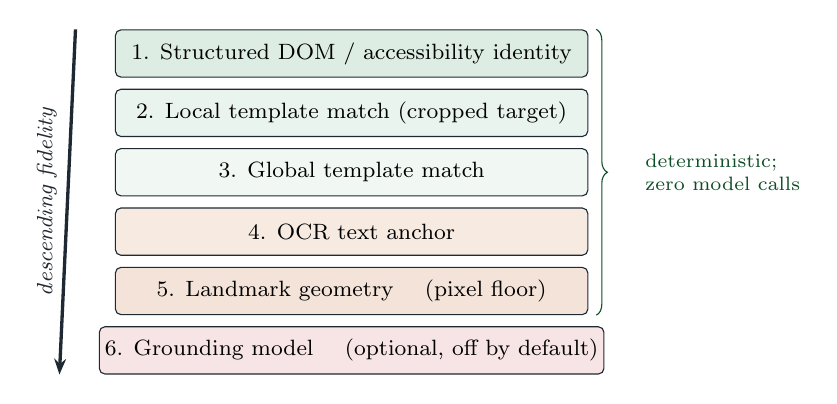
\begin{tikzpicture}[
  font=\footnotesize,
  rung/.style={draw=oaink, rounded corners=2pt, minimum width=60mm,
    minimum height=6mm, align=center, inner sep=2pt},
  ]
  \node[rung, fill=oagreen!14] (r1) {1. Structured DOM / accessibility identity};
  \node[rung, fill=oagreen!9, below=1.4mm of r1] (r2) {2. Local template match (cropped target)};
  \node[rung, fill=oagreen!6, below=1.4mm of r2] (r3) {3. Global template match};
  \node[rung, fill=oaamber!12, below=1.4mm of r3] (r4) {4. OCR text anchor};
  \node[rung, fill=oaamber!16, below=1.4mm of r4] (r5) {5. Landmark geometry \quad (pixel floor)};
  \node[rung, fill=oared!12, below=1.4mm of r5] (r6) {6. Grounding model \quad (optional, off by default)};
  \draw[-{Stealth[length=2mm]}, very thick, oaink]
    ($(r1.north west)+(-5mm,0)$) -- ($(r6.south west)+(-5mm,0)$)
    node[midway, rotate=90, anchor=south, font=\footnotesize\itshape]{descending fidelity};
  \draw[decorate, decoration={brace, amplitude=4pt}, oagreen!60!black]
    ($(r1.north east)+(1mm,0)$) -- ($(r5.south east)+(1mm,0)$);
  \node[right=6mm of r3, align=left, font=\scriptsize, text=oagreen!60!black]
    {deterministic;\\zero model calls};
\end{tikzpicture}
\caption{The resolution ladder tries evidence in descending order of fidelity.
Rungs 1--5 are deterministic and make no model calls; a grounding model is an
optional last rung, off by default and still subject to the same identity and
effect checks.}
\label{fig:ladder}
\end{figure}

\section{Related work}
\label{sec:related}

\paragraph{Computer-use agents and their benchmarks.} Recent agents observe the
screen and choose actions with a general multimodal model
\cite{anthropic2024computeruse,uitars2025,cheng2024seeclick}, evaluated on
breadth-oriented suites \cite{webarena,workarena,osworld}. Their oracles are
task-completion checks read from the interface. Our contribution is orthogonal
and composable: we do not propose a better agent but a stronger reliability
metric and a verifier that any of these systems could adopt for consequential
steps.

\paragraph{RPA, visual scripting, and programming by demonstration.} Robotic
process automation executes deterministic rules over existing interfaces
\cite{vanderaalst2018rpa}; visual scripting made screenshot patterns a
first-class interface \cite{sikuli}; and programming-by-demonstration and
by-example infer reusable programs from user actions
\cite{cypher1993watch,gulwani2011automating,chasins2018rousillon}. These deliver
determinism and reuse but, like the agents, typically confirm success from the
screen. \system{} inherits the deterministic-replay idea and adds runtime repair
under drift and, centrally here, verification of the downstream effect.

\paragraph{Oracles and end-to-end effects.} Choosing what makes an outcome
correct is the test-oracle problem \cite{barr2015oracle}; the end-to-end argument
locates the check at the layer that establishes the property \cite{saltzer1984end};
and the faults we target are classical transactional hazards
\cite{gray1981transaction}. We apply these ideas to GUI automation, where the
prevailing oracle is a screenshot.

\section{Result: screen-only verification silently accepts wrong effects}
\label{sec:faults}

\paragraph{Design.} We inject seven persistence faults, plus two controls, at a
real HTTP persistence boundary behind a browser triage workflow, with ten repeats
per class. The oracle is database state, not the UI report. Each class is
evaluated twice through the live replayer: once with screen-only verification,
and once with a declared typed effect and a system-of-record verifier configured.
We report silent incorrect success (the runtime reports success while the
external oracle disagrees) and false abort (the effect occurred but the runtime
reports failure).

\paragraph{Finding.} Under screen-only verification, silent wrong effects are the
common case, not a corner case: replay silently accepted 50 of 90 fault runs and
falsely aborted 10 correct ones. Adding a system-of-record effect check reduced
both to zero (Figure~\ref{fig:silentbar}). Broken out by class, screen-only
verification silently mishandled five of seven injected fault classes: partial
save, duplicate submission, optimistic UI followed by rejection, stale overwrite,
and double delivery. There were 10 consistent repeats per class. When the step
declared the expected effect and a system-of-record verifier was configured,
those five classes refuted and halted through the live replayer.

\begin{figure}[t]
\centering
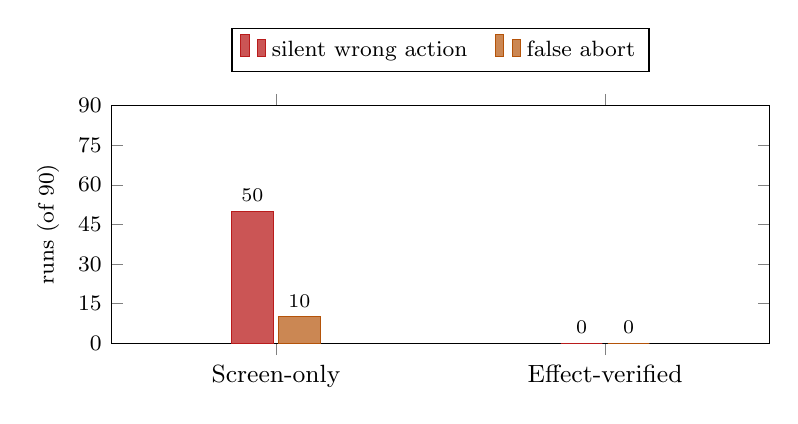
\begin{tikzpicture}
\begin{axis}[
  ybar,
  bar width=15pt,
  width=0.82\linewidth,
  height=4.6cm,
  ymin=0, ymax=90,
  ylabel={runs (of 90)},
  ylabel style={font=\footnotesize},
  symbolic x coords={Screen-only, Effect-verified},
  xtick=data,
  xticklabel style={font=\small},
  ytick={0,15,30,45,60,75,90},
  yticklabel style={font=\footnotesize},
  enlarge x limits=0.5,
  legend style={font=\footnotesize, at={(0.5,1.14)}, anchor=south,
    legend columns=-1, /tikz/every even column/.append style={column sep=8pt}},
  nodes near coords, nodes near coords style={font=\scriptsize},
]
\addplot[fill=oared!75, draw=oared] coordinates {(Screen-only,50) (Effect-verified,0)};
\addplot[fill=oaamber!70, draw=oaamber] coordinates {(Screen-only,10) (Effect-verified,0)};
\legend{silent wrong action, false abort}
\end{axis}
\end{tikzpicture}
\caption{Same 90 injected-fault runs, two verification policies. Screen-only
verification---the signal task-success oracles read---silently accepted 50 wrong
outcomes and falsely aborted 10 correct ones; a system-of-record effect check
reduced both to zero. Two preconditions are non-optional: the effect must be
authored and the verifier deployed.}
\label{fig:silentbar}
\end{figure}

\begin{table}[t]
\centering
\caption{Per-class outcomes for the seven injected faults (ten repeats each),
under screen-only verification and under a system-of-record effect verifier.
\emph{Silent} marks a run the screen reported as success while the database
disagreed. Two idempotent/clean controls (not shown) succeed under both.}
\label{tab:faults}
\small
\begin{tabular}{lll}
\toprule
Injected fault & Screen-only outcome & Effect verdict \\
\midrule
Partial save            & \textcolor{oared}{silent success} & refuted (halt) \\
Duplicate submission    & \textcolor{oared}{silent success} & refuted (halt) \\
Optimistic then reject  & \textcolor{oared}{silent success} & refuted (halt) \\
Stale overwrite         & \textcolor{oared}{silent success} & refuted (halt) \\
Double delivery         & \textcolor{oared}{silent success} & refuted (halt) \\
Timeout after commit    & false abort                        & confirmed \\
Session loss            & safe halt                          & refuted (halt) \\
\bottomrule
\end{tabular}
\end{table}

\paragraph{Reading.} The improvement is not a model, a bigger prompt, or a
retry policy. It is a change of oracle. The precondition is real work: the
expected effect must be authored per deployment and the verifier configured, and
the compiler does not yet infer effects from a single demonstration. But the
result isolates the metric problem cleanly. On these classes, a task-success
oracle would have scored the screen-only runs as successes fifty times while the
database disagreed.

\section{Supporting result: refuse rather than guess on ambiguous identity}
\label{sec:identity}

The same principle---do not trust an under-determined observation---appears at the
identity layer, and it is where a naive fix (trust the screen harder) is most
dangerous. Target resolution answers \emph{where} to act; identity verification
asks \emph{whether} the resolved target is the intended entity. On a dense list of
records that share a name and date of birth, distinguished only by confusable
glyphs such as O against 0 or l against 1, OCR can make two distinct identifiers
observationally identical. The safe response on an unreadable identifier is to
abstain and halt, not to click.

We evaluate the integrated replayer against adversarial homonyms in structured and
pure-pixel configurations, and report both false accept and over-halt, because a
system can trivially reach zero wrong clicks by refusing every correct one. The
identity ladder recorded zero false accepts in every tested configuration.
Structured browser identity additionally had zero over-halts on 14 correct homonym
cases. Pure-pixel configurations halted on all correct confusable cases: zero
false accepts at 100\% over-halt---the intended safety/availability disclosure,
not evidence that pixel-only identity is ready for dense clinical lists. The
point for this venue is the asymmetry: a wrong write to a look-alike record is
unrecoverable, so an honest system pays availability to buy the guarantee that it
never silently acts on a target it cannot verify.

\section{Scope and what this does not show}
\label{sec:scope}

These are bounded studies. The fault model is a deterministic mechanism study at
one persistence boundary, not a population estimate over enterprise applications;
the identity study uses synthetic adversarial homonyms; effect verifiers require
per-deployment authoring. We make no claim here about long-term reliability,
maintenance cost, or clinical-production safety, and no measured result covers
Citrix ICA/HDX. The full report adds a repeated-workflow latency and cost
comparison against a computer-use agent, a public-web breadth corpus, a
drift-repair study, and scoped qualifications of native Windows UIA, macOS, and
real-network RDP substrates, each with an independent effect oracle. The authors
develop the evaluated system; raw artifacts and scripts reduce but do not
eliminate experimenter bias, and independent replication remains necessary.

\section{Recommendations for evaluating GUI agents}
\label{sec:recs}

We distill the position into four concrete practices for benchmark and system
designers.
\begin{enumerate}
  \item \textbf{Report silent incorrect success.} For any task with a persisted
        effect, score the run against an oracle that reads the system of record,
        not the final screen, and publish the rate at which the agent reported
        success while that oracle disagreed.
  \item \textbf{Report over-halt, not only success.} Safety that is bought by
        refusing available correct actions is not free. Pair every refusal claim
        with the rate of refusing when the correct action was in fact available,
        so a benchmark cannot be gamed by abstaining.
  \item \textbf{Separate delivery from effect.} A clean return code, a settled
        screenshot, and a confirmation banner attest to \emph{delivery}. Treat
        them as necessary conditions and verify the \emph{effect} independently.
  \item \textbf{Publish per-class outcomes.} Aggregate success rates hide the
        exact failure that matters. A single silently mishandled fault class,
        repeated, is more informative than a high mean.
\end{enumerate}
These practices are inexpensive relative to building the agent, and they change
which systems look reliable. Under a task-success oracle the screen-only runs in
Section~\ref{sec:faults} score as fifty additional successes; under an
effect oracle they score as fifty caught faults.

\section{Conclusion}
\label{sec:conclusion}

Task success is a breadth metric that quietly assumes the screen tells the truth.
For repeated, consequential GUI work it does not: a green banner is not a saved
record, and screen-only verification silently accepted more than half of our
injected fault runs. The remedy is not a better model but a better oracle---verify
the declared effect against the system of record, and refuse when identity or
effect cannot be verified. We recommend that benchmarks for computer-use and GUI
agents report silent incorrect success and over-halt against an independent
oracle alongside task success. The mechanism that makes such checks the
exceptional event---a demonstration compiler with deterministic replay and
governed repair---is described in full in the \fullreport{}.

% paper/workshop/references.bib is a byte-identical copy of ../references.bib
% (kept a regular file, NOT a symlink, so it packages cleanly in the sdist); the
% workshop shares the full report's single bibliography. check_artifacts.py
% asserts the two files stay identical so they cannot silently drift.
\bibliographystyle{plain}
\bibliography{references}

\end{document}
